%-----------------------------------------------------------------------------%
\chapter{\babDua}
%-----------------------------------------------------------------------------%
Bagian ini menjelaskan teori-teori yang digunakan dalam penelitian. Teori yang dimaksud adalah pengetahuan yang terkait dengan pelaksanaan penelitian.

%-----------------------------------------------------------------------------%
\section{Deep Learning}
%-----------------------------------------------------------------------------%7
\textit{Deep Learning} merupakan salah satu bentuk \textit{Representation Learning} yang memungkinkan suatu mesin untuk diberikan sekumpulan data mentah, kemudian mesin tersebut dapat secara otomatis menemukan representasi data (\textit{feature vector}) yang diperlukan untuk melakukan klasifikasi atau deteksi. \textit{Deep Learning} dikenal memiliki akurasi yang lebih tinggi daripada algoritma \textit{Machine Learning} konvensional dalam melakukan klasifikasi atau deteksi. \textit{Deep Learning} memanfaatkan arsitektur \textit{Neural Network} sebagai model. Arsitektur ini terinspirasi dari otak manusia yang terdiri dari banyak neuron. Model \textit{Deep Learning} dilatih menggunakan sekumpulan data yang telah diketahui labelnya. Oleh karena itu, \textit{Deep Learning} merupakan salah satu bentuk dari \textit{Supervised Learning} \cite{deeplearning}. 

Contoh model \textit{Deep Learning} yang sangat terkenal adalah \textit{Convolutional Neural Network} (CNN). CNN didesain untuk memproses data berupa \textit{multi-dimensional array}, contohnya data citra. CNN sering digunakan dalam aplikasi pengenalan citra dan deteksi objek pada citra. CNN tersusun dari beberapa \textit{convolution layer} yang berfungsi untuk mengekstrak fitur-fitur dari data dengan cara melakukan konvolusi menggunakan suatu \textit{filter} \cite{deeplearningmatrix}. \textit{Convolution layer} biasanya disambungkan ke \textit{pooling layer}, yaitu \textit{layer} yang berfungsi untuk mereduksi ukuran matriks dengan cara melakukan \textit{downsampling}. Pada bagian akhir model biasanya juga terdapat \textit{fully-connected layer} yang bertugas melakukan klasifikasi menggunakan fitur-fitur yang didapat dari proses konvolusi pada \textit{convolution layer}. \pic~\ref{fig:cnn} merupakan contoh model CNN.

\begin{figure}
	\centering
	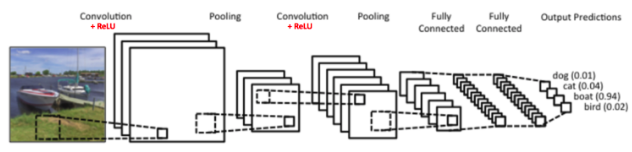
\includegraphics[width=0.50\textwidth]
	{pics/cnn.png}
	\caption{Contoh model Convolutional Neural Network (CNN). Pada model ini terdapat \textit{convolution layer}, \textit{pooling layer}, dan \textit{fully-connected layer}.}
	\label{fig:cnn}
\end{figure}

%-----------------------------------------------------------------------------%
\section{Deep Learning Training dan Inference}
%-----------------------------------------------------------------------------%
\textit{Deep Learning} merupakan algoritma yang terdiri dari dua tahap, yaitu \textit{training} dan \textit{inference}. Pada tahap \textit{training}, model dilatih menggunakan sekumpulan data. Pada awal \textit{training}, \textit{weight} inisial diberikan kepada model, biasanya berupa angka-angka acak berdasarkan suatu distribusi tertentu. Selanjutnya, data training dimasukkan ke model. Model melakukan \textit{forward pass} atau prediksi terhadap data tersebut menggunakan \textit{weight} sehingga akan diperoleh skor atau label dari data pada \textit{output layer}. Label hasil prediksi kemudian dibandingkan dengan label asli dari data dan dihitung nilai galatnya menggunakan fungsi tertentu. Informasi galat ini kemudian dikirim kembali ke semua \textit{layer} pada model dan digunakan untuk memperbarui nilai \weight pada tiap \textit{layer}. Proses mengirim kembali informasi galat ini disebut \textit{back propagation} \cite{trainvsinfer}. 

Model yang telah dilatih pada tahap \textit{training} dapat digunakan untuk melakukan \textit{inference}. \textit{Inference} merupakan tahap dimana model melakukan \textit{forward pass} terhadap data baru menggunakan model yang telah dilatih. Perbedaan utama dari \textit{training} dan \textit{inference} adalah bahwa pada \textit{inference} tidak terdapat \textit{back-propagation} setelah melakukan \textit{forward-pass}, karena tujuan dari \textit{inference} hanyalah mendapatkan hasil prediksi skor atau label dari data baru \cite{trainvsinfer}. \pic~\ref{fig:trainvsinfer} menunjukkan perbedaan proses \textit{training} dan \textit{inference}. Terlihat bahwa pada \textit{training} terjadi pemrosesan dua arah, sedangkan pada \textit{inference} hanya satu arah.

\begin{figure}
	\centering
	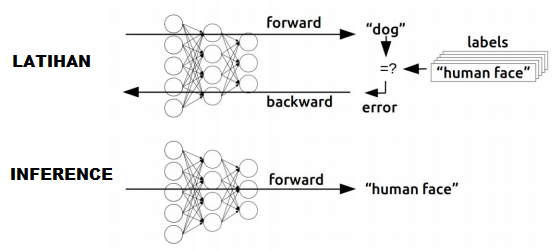
\includegraphics[width=0.50\textwidth]
	{pics/trainingvsinference.png}
	\caption{Perbedaan \textit{training} dan \textit{inference} pada \textit{Deep Learning}. \textit{Training} merupakan proses dua arah, sedangkan \textit{inference} hanya satu arah.}
	\label{fig:trainvsinfer}
\end{figure}

\section{Operasi-operasi Deep Learning Inference}
%-----------------------------------------------------------------------------%
Tahap \textit{inference} pada \textit{Deep Learning} melibatakan banyak operasi-operasi matriks. Konvolusi matriks dan perkalian matriks-matriks merupakan beberapa operasi pada \textit{Deep Learning} \textit{inference} yang memiliki beban komputasi besar. Dua operasi ini merupakan dua operasi yang diamati pada penelitian ini. Berikut adalah penjelasan lebih lanjut mengenai tiga operasi tersebut.

\subsection{Konvolusi Matriks}
Operasi konvolusi matriks terjadi pada \textit{convolution layer} dari CNN. Operasi ini melibatkan tiga buah matriks yaitu matriks \textit{image}, matriks \textit{filter}, dan matriks \textit{output}. Matriks-matriks tersebut memiliki tiga dimensi yang merepresentasikan kanal, baris, dan kolom. Kanal adalah sumbu-z dari matriks. Banyaknya kanal menyatakan kedalaman matriks. Baris merupakan sumbu-y dari matriks. Banyaknya baris menyatakan ketinggian matriks. Kolom merupakan sumbu-x dari matriks. Banyaknya kolom menyatakan lebar matriks.

Pada \textit{convolution layer}, \textit{filter} dikonvolusikan terhadap matriks \textit{image}. Suatu \textit{image} dapat dikonvolusi menggunakan satu atau lebih \textit{filter}. Karena itu, \textit{filter} sebenarnya adalah matriks empat dimensi yaitu kanal, baris, kolom, dan \textit{batch}. Besarnya \textit{batch} menyatakan banyaknya \textit{filter} tiga dimensi kanal, baris, dan kolom. Konvolusi dari satu \textit{batch} dari \textit{filter} menghasilkan satu kanal tersendiri pada matriks \textit{output}, sehingga besarnya \textit{batch} dari \textit{filter} akan selalu sama dengan banyaknya kanal (kedalaman) \textit{output} \cite{deeplearningmatrix}. Berikut adalah beberapa aturan mengenai ukuran matriks \textit{image}, \textit{filter}, \textit{bias}, dan \textit{output} pada convolution layer. 

\begin{enumerate}
\item Tinggi dan lebar \textit{filter} selalu lebih kecil atau sama dengan tinggi dan lebar \textit{image}.
\item Kedalaman \textit{image} selalu sama dengan kedalaman \textit{filter}.
\item Besarnya \textit{batch} selalu sama dengan kedalaman \textit{output}.
\item Tinggi dan lebar \textit{bias} selalu sama dengan satu.
\item Kedalaman \textit{bias} selalu sama dengan kedalaman \textit{output}.
\item Tinggi dan lebar \textit{output} selalu lebih kecil atau sama dengan tinggi dan lebar \textit{image}.
\end{enumerate}	

Pada operasi konvolusi, posisi \textit{filter} dimulai dari ujung kiri atas dari \textit{image}. \textit{Filter} kemudian bergeser ke kanan dan kebawah dengan jarak geser (\textit{stride}) yang ditentukan (pada umumnya \textit{stride} sama dengan satu). Pada suatu posisi \textit{filter}, dilakukan \textit{dot-product} antara \textit{filter} dengan sub-matriks dari \textit{image} yang bersesuaian dengan posisi filter. Satu kali operasi \textit{dot-product} tersebut menghasilkan skalar yang merupakan satu elemen dari matriks \textit{output} setelah ditambahkan bias dan diaktivasi. Setelah proses konvolusi selesai untuk satu \textit{filter}, akan terbentuk satu kanal \textit{output}. \pic~\ref{fig:conv} menunjukkan contoh operasi konvolusi dengan \textit{image} berukuran $5 \times 5 \times 1$, \textit{filter} berukuran $3 \times 3 \times 1$, dan nilai \textit{stride} satu.

\begin{figure}
	\centering
	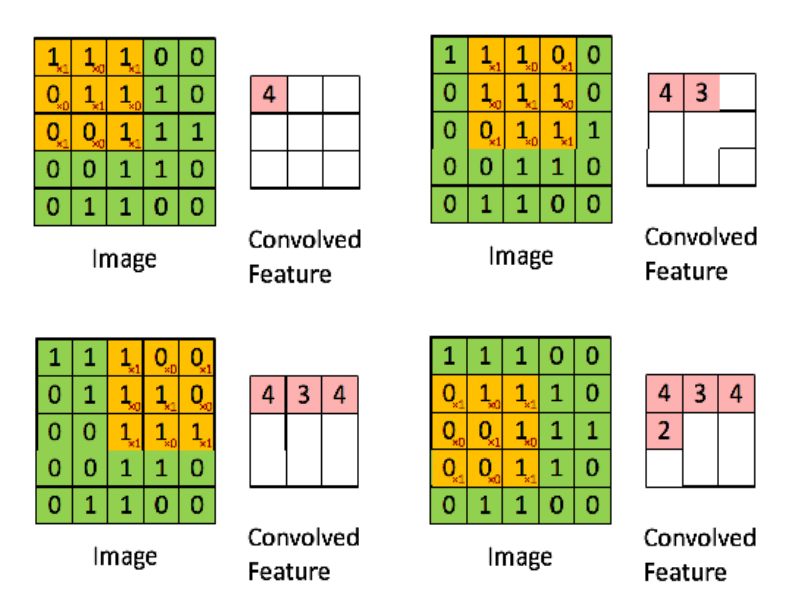
\includegraphics[width=0.50\textwidth]
	{pics/conv.png}
	\caption{Contoh operasi konvolusi. \textit{Convolved feature} adalah matriks keluaran dari konvolusi.}
	\label{fig:conv}
\end{figure}

Operasi konvolusi seperti di atas dapat dilakukan sekaligus untuk beberapa \textit{batch}. Jika \textit{batch} lebih dari satu, maka matriks-matriks \textit{image} dan \textit{output} adalah matriks empat dimensi yaitu kanal, baris, kolom, dan \textit{batch}. 

\subsection{Perkalian Matriks-Matriks}
Operasi perkalian matriks-matriks pada \textit{Deep Learning inference} terjadi pada \textit{fully-connected layer}. Pada \textit{layer} ke-\textit{l}, nilai \textit{weight} disimpan dalam bentuk matriks dua dimensi berukuran $M \times K$, dimana $M$ adalah banyaknya \textit{node} pada \textit{layer} ke-\textit{l} dan $K$ adalah banyaknya \textit{node} pada \textit{layer} ke-\textit{(l-1)} \cite{deeplearningmatrix}. Baris ke-\textit{i} dari matriks \textit{weight} pada \textit{layer} ke-\textit{l} tersebut merupakan vektor \textit{weight} untuk \textit{node} ke-\textit{i} pada \textit{layer} ke-\textit{l}. Untuk memperoleh nilai semua \textit{node} pada \textit{layer} ke-\textit{l}, matriks \textit{weight} dikalikan dengan vektor sepanjang $K$ yang elemen-elemennya adalah nilai-nilai \textit{node} pada \textit{layer} ke-\textit{(l-1)}. Hasilnya adalah vektor sepanjang $M$, sesuai banyaknya \textit{node} pada \textit{layer} ke-\textit{l}. Ini dapat dilihat pada \pic~\ref{fig:fcmatmul}. 

\begin{figure}
	\centering
	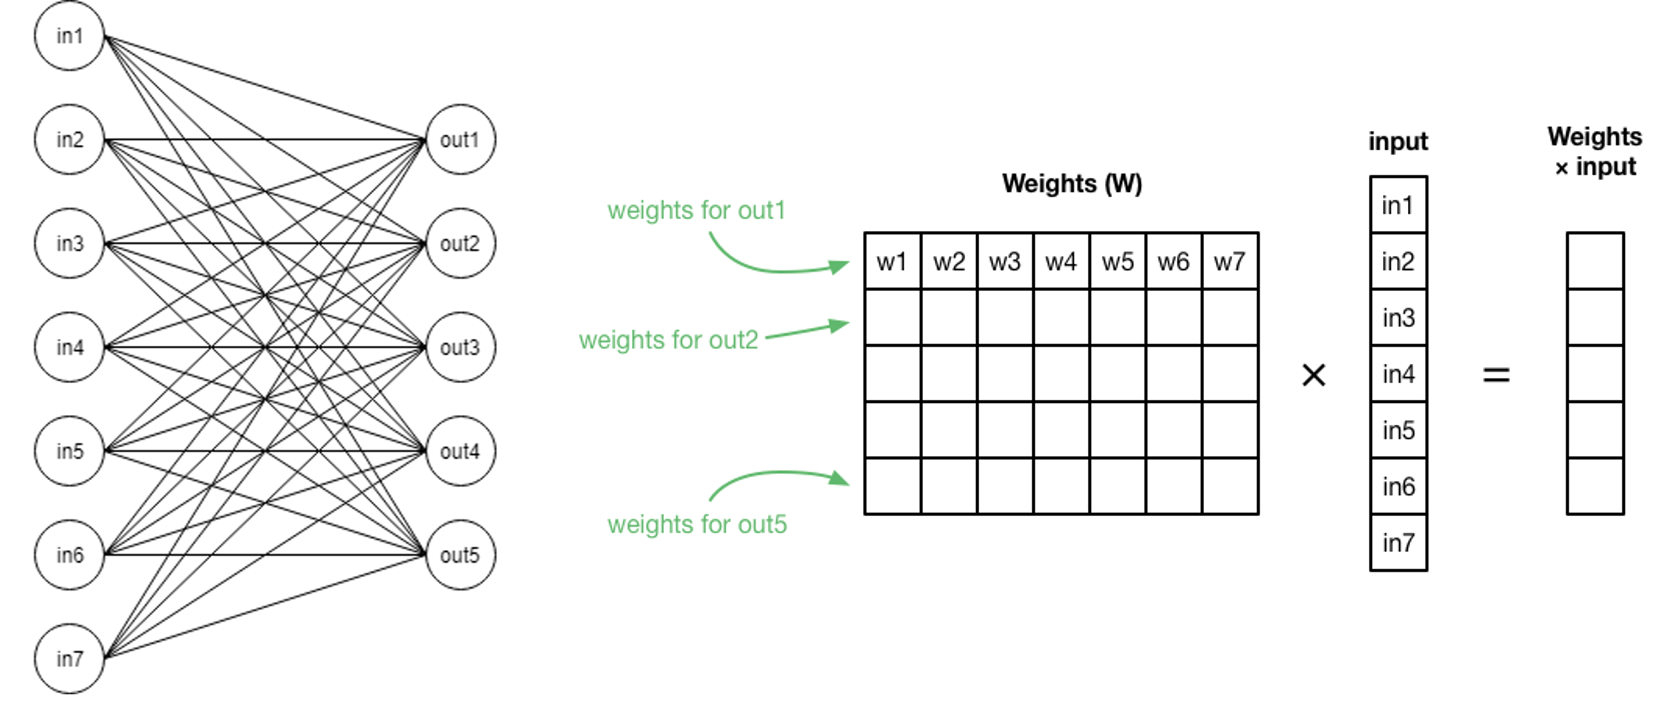
\includegraphics[width=0.50\textwidth]
	{pics/fcmatmul.png}
	\caption{Perkalian matriks-vektor pada \textit{fully-connected layer}. Elemen ke-$i$ pada vektor \textit{weightxinput} adalah nilai $outi$.}
	\label{fig:fcmatmul}
\end{figure}

Operasi perkalian matriks $M \times K$ dengan vektor $K \times 1$ pada \textit{fully-connected layer} tersebut dapat dilakukan sekaligus untuk $N$ \textit{batch}, sehingga akan terjadi operasi perkalian matriks $M \times K$ dengan matriks $K \times N$ yang menghasilkan matriks $M \times N$.

Selain \textit{fully-connected layer}, operasi perkalian matriks-matriks juga dapat terjadi pada \textit{convolution layer}. Terdapat dua kasus yang menyebabkan terjadinya operasi ini. Kasus pertama adalah ketika operasi konvolusi melibatkan \textit{filter} yang berukuran tinggi dan lebar $1 \times 1$. \textit{Image} dapat dipandang sebagai matriks dua dimensi dengan tinggi $H_{i} \times W_{i} \times B_{i}$ dan lebar $C_{i}$ dimana $H_{i}$, $W_{i}$, $C_{i}$, dan $B_{i}$ berturut-turut adalah tinggi, lebar, banyaknya kanal, dan banyaknya \textit{batch} dari \textit{image}. Sementara itu \textit{filter} dapat dipandang sebagai matriks dua dimensi dengan tinggi $C_{f}$ dan lebar $H_{f} \times W_{f} \times B_{f}$ dimana $H_{f}$, $W_{f}$, $C_{f}$, dan $B_{f}$ berturut-turut adalah tinggi, lebar, banyaknya kanal, dan banyaknya \textit{batch} dari \textit{filter}.

Kasus kedua terjadinya perkalian matriks-matriks pada \textit{convolution layer} adalah ketika operasi konvolusi melibatkan \textit{filter} yang tinggi dan lebarnya sama dengan tinggi dan lebar \textit{image}. \textit{Image} dapat dipandang sebagai matriks dua dimensi dengan tinggi $B_{i}$ dan lebar $H_{i} \times W_{i} \times C_{i}$, sedangkan \textit{filter} dapat dipandang sebagai matriks dua dimensi dengan tinggi $H_{f} \times W_{f} \times C_{f}$ dan lebar $B_{f}$.

\section{Tensorflow Lite}
%-----------------------------------------------------------------------------%
TensorFlow \cite{tensorflow} adalah perangkat lunak \textit{open-source} yang merupakan \textit{library} untuk melakukan komputasi numerik menggunakan graf. \textit{Node} pada graf merepresentasikan operasi matematika, sedangkan \textit{edge} pada graf merepresentasikan \textit{multidimensional data array} (\textit{tensor}) sebagai masukan atau keluaran dari operasi pada \textit{node}. TensorFlow pada awalnya dikembangkan oleh para pengembang dan peneliti dari Google untuk keperluan penelitian di bidang \textit{Machine Learning} and \textit{Deep Learning}. Saat ini Tensorflow merupakan salah satu \textit{Machine Learning library} paling populer. API Tensorflow tersedia dalam bahasa C++, Python, Java, dan Javascript. Selain digunakan pada komputer personal atau \textit{server}, Tensorflow juga dapat digunakan untuk menjalankan \textit{Deep Learning inference} pada perangkat \textit{mobile} melalui Tensorflow Mobile dan Tensorflow Lite.

Tensorflow Lite merupakan \textit{Machine Learning library} terbaru dari Tensorflow yang ditujukan untuk perangkat Android dan IoS \cite{tflite}. Saat ini Tensorflow Lite dapat memproses tiga jenis model \textit{Deep Learning} yaitu CNN, DNN, dan LSTM. Berbeda dengan Tensorflow Mobile, Tensorflow Lite memiliki \textit{kernel} tersendiri yang terpisah dari \textit{core} Tensorflow. \textit{Kernel} adalah implementasi operasi-operasi \textit{Deep Learning infernce} seperti perkalian matriks, konvolusi, dan transpose matriks. Tensorflow Lite memiliki suatu jenis \textit{kernel} yang telah dioptimalkan untuk perangkat \textit{mobile} (\textit{optimized kernel}) yang memiliki performa yang sangat baik. Selain \textit{optimized kernel}, terdapat pula \textit{kernel} biasa (\textit{naive kernel}) pada Tensorflow Lite. Namun tentu saja performanya tidak lebih baik dari \textit{optimized kernel}.

Untuk melakukan \textit{inference}, Tensorflow Lite menerima masukan model dengan format ".tflite". API akan meneruskan model masukan ke \textit{interpreter} untuk diinterpretasi. \textit{Interpreter} akan memuat semua \textit{kernel} yang diperlukan oleh model tersebut secara selektif. \pic~\ref{fig:tflite} menjelaskan arsitektur Tensorfow Lite.

\begin{figure}
	\centering
	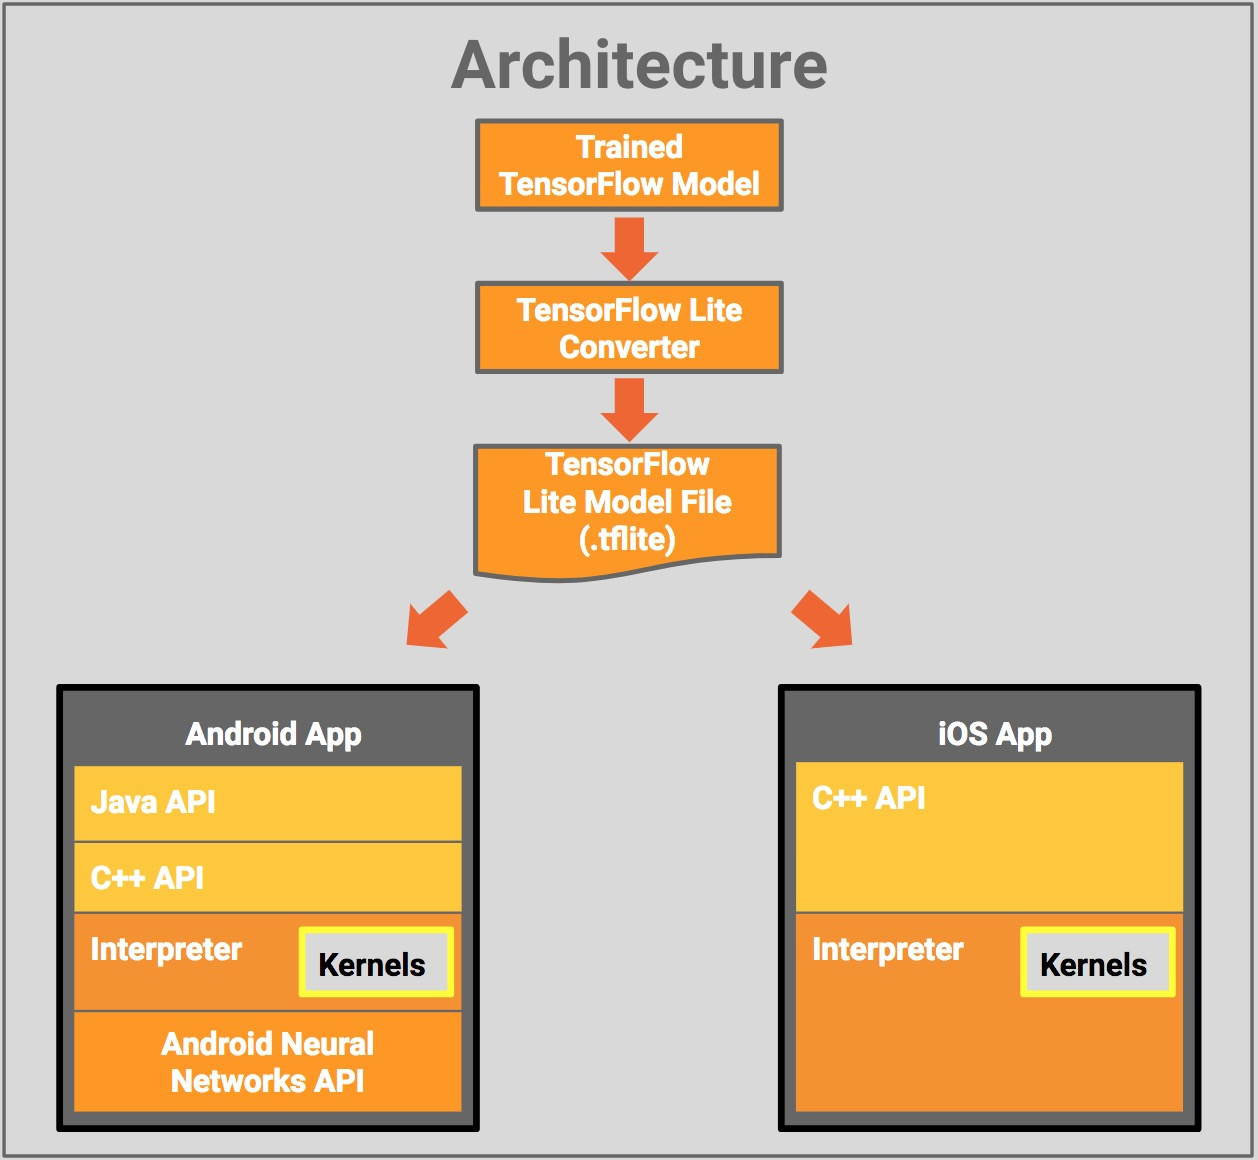
\includegraphics[width=0.50\textwidth]
	{pics/tflite.jpg}
	\caption{Arsitektur Tensorflow Lite. \textit{Interpreter} bertugas menginterpretasikan model ".tflite" dan memuat \textit{kernels} yang diperlukan. \textit{Kernels} tersebut terpisah dari \textit{core} Tensorflow.}
	\label{fig:tflite}
\end{figure}

\section{OpenCL}
%-----------------------------------------------------------------------------%
OpenCL merupakan API untuk melakukan pemrograman paralel pada prosesor yang berbeda-beda seperti CPU, GPU, DSP, dan FPGA \cite{opencl}. OpenCL dapat digunakan untuk meningkatkan performa komputasi secara signifikan. OpenCL API menggunakan bahasa C/C++ dengan ekstensi. Pada OpenCL terdapat dua sisi program, yaitu \textit{host} dan \textit{device}. \textit{Device} adalah prosesor target, tempat berjalannya komputasi. Sementara itu \textit{host} adalah yang mengatur jalannya komputasi pada \textit{device}. Menyalin data matriks dari \textit{host memory} ke \textit{device memory} dan menentukan banyaknya unit komputasi yang bekerja adalah contoh tugas dari \textit{host}. Dalam penelitian ini program \textit{host} berjalan pada CPU. \textit{Device} pada penelitian ini adalah GPU. Dalam suatu program OpenCL terdapat istilah-istilah yang perlu dipahami sebagai berikut.

\begin{enumerate}
	\item \textbf{\textit{Context}}. \textit{Context} adalah lingkungan dimana komputasi pada \textit{device} akan dilakukan. Pada \textit{context} didefiniskan OpenCL \textit{kernel} yang digunakan, \textit{device} yang digunakan, memori (\textit{buffer}) yang dapat diakses, properti dari memori tersebut, dan satu atau lebih \textit{command queue} untuk penjadwalan eksekusi OpenCL \textit{kernel}.
	
	\item \textbf{\textit{Kernel}}. OpenCL \textit{kernel} merupakan serangkaian instruksi yang mendefinisikan suatu fungsi tertentu, contohnya perkalian matriks atau penjumlahan matriks, yang dieksekusi pada \textit{device}. OpenCL \textit{kernel} dikompilasi dan dijadwalkan eksekusinya oleh \textit{host}. OpenCL \textit{kernel} pada bagian \textit{host} direpresentasikan dalam format \textit{string} dan dikompilasi menggunakan fungsi $clBuildKernel()$ pada OpenCL API.
	
	\item \textbf{\textit{Buffer}}. \textit{Buffer} atau \textit{buffer object} merupakan \textit{memory object} yang menyimpan koleksi data secara linear dalam \textit{bytes}. \textit{Buffer} berada pada \textit{device memory} (dalam penelitian ini adalah memori GPU). OpenCL \textit{kernel} dapat mengakses data pada \textit{buffer} menggunakan \textit{pointer} yang diberikan melalui argumen \textit{kernel}. Data pada \textit{buffer} juga dapat dimanipulasi oleh \textit{host}.
	
	\item \textbf{\textit{Command Queue}}. \textit{Command queue} merupakan objek yang menampung perintah-perintah yang akan dieksekusi pada \textit{device}.
\end{enumerate}

Tahap-tahap berjalannya suatu program OpenCL dapat dilihat pada \tab~\ref{tab:OpenCLexecutionorder}. Sebelum suatu OpenCL \textit{kernel} dapat dieksekusi pada \textit{device}, \textit{host} perlu melakukan beberapa persiapan seperti pada \tab~\ref{tab:OpenCLexecutionorder}. Ketika persiapan telah selesai, OpenCL \textit{kernel} dapat dijadwalkan eksekusinya dengan cara melakukan \textit{enqueue} terhadap \textit{command queue}. Perhatikan bahwa data-data yang terkait dengan eksekusi OpenCL \textit{kernel} (data masukan dan data keluaran) perlu disalin secara manual dari \textit{host memory} (CPU) ke \textit{device memory} (GPU) dan sebaliknya.

\begin{table}
	\centering
	\caption{Tahap-tahap eksekusi program OpenCL dari awal hingga akhir.}
	\label{tab:OpenCLexecutionorder}
	\begin{tabular}{| l | l |}
		\hline
		\textbf{No.} & \textbf{Tahap}\\ 
		\hline
		1 & Membuat \textit{context} \\ 
		\hline 
		2 & Membuat \textit{kernel}\\ 
		\hline 
		3 & Membuat \textit{comand-queue}\\ 
		\hline
		4 & Membuat \textit{buffer}\\ 
		\hline
		5 & Menyalin data masukan dari \textit{host memory} ke \textit{device memory}.\\
		\hline
		6 & Mendefinisikan struktur \textit{work-space}.\\
		\hline
		7 & Mendefinisikan argumen-argumen \textit{kernel}.\\
		\hline
		8 & Eksekusi \textit{kernel}. \\
		\hline
		9 & Menyalin data keluaran dari 
		\textit{device memory} ke \textit{host memory}. \\
		\hline
	\end{tabular}
\end{table}				

Untuk mengimplementasikan OpenCL, diperlukan OpenCL \textit{library} ("libOpenCL.so") dan OpenCL \textit{headers} ("cl.h" dan "cl\_platform.h"). Pada NVIDIA GPU, OpenCL \textit{library} dapat diperoleh dalam paket instalasi CUDA. Pada perangkat Android, OpenCL \textit{library} disediakan oleh vendor dari masing-masing prosesor. Perangkat Android dengan vendor GPU Adreno atau Mali biasanya menyertakan OpenCL \textit{library} yang terletak pada direktori "/system/vendor/lib/". \textit{Library} tersebut dapat diambil menggunakan perintah "adb pull" pada Linux.

\section{SIMT pada OpenCL}
%-----------------------------------------------------------------------------%
GPU merupakan prosesor yang memiliki banyak unit komputasi (\textit{thread}). Melalui OpenCL, komputasi pada GPU dapat dijalankan oleh banyak \textit{thread} yang bekerja secara paralel, sehinnga dapat meningkatkan kecepatan komputasi. Konsep paralelisasi pada OpenCL pada dasarnya adalah semua \textit{thread} menjalakan instruksi yang sama, namun bagian data yang diproses oleh masing-masing \textit{thread} berbeda-beda. Misalnya operasi penjumlahan dua vektor sepanjang $N$ dapat dikerjakan oleh $N$ \textit{thread}, dimana \textit{thread} ke-\textit{i} hanya menjumlahkan elemen ke-\textit{i} dari dua vektor tersebut. Pada OpenCL, unit komputasi atau \textit{thread} ini disebut \textit{work-item} \cite{opencl}. 

OpenCL \textit{kernel} dieksekusi dalam suatu \textit{work-space} yang terdiri dari sekumpulan \textit{work-item} yang membentuk struktur satu hingga tiga dimensi. Pada suatu \textit{work-space}, semua \textit{work-item} mengeksekusi OpenCL \textit{kernel} yang sama. \textit{Work-space} dapat dibagi ke dalam beberapa \textit{work-group}. \textit{Work-group} terdiri dari beberapa \textit{work-item} yang membentuk blok satu hingga tiga dimensi. Secara umum, seluruh \textit{work-item} pada \textit{work-space} bekerja secara independen, namun sinkronisasi dapat dilakukan antar \textit{work-item} yang berada pada \textit{work-group} yang sama.

Setiap \textit{work-item} memiliki \textit{identifier} (ID) yang unik. ID adalah bilangan bulat yang lebih besar dari atau sama dengan nol. Setiap \textit{work-item} memiliki dua jenis ID, yaitu \textit{global} ID dan \textit{local} ID. \textit{Global} ID mengidentifikasi \textit{work-item} dalam suatu \textit{work-space}, sedangkan \textit{local} ID mengidentifikasi \textit{work-item} dalam suatu \textit{work-group}. Setiap \textit{work-group} juga memiliki ID yang unik. Saat suatu proses berjalan pada \textit{device}, ID dari \textit{work-item} dan \textit{work-group} yang menjalankan proses tersebut dapat diambil. ID tersebut dapat dimanfaatkan untuk mengatur paralelisasi dari eksekusi OpenCL \textit{kernel}. \pic~\ref{fig:work} adalah contoh \textit{work-space} dua dimensi pada OpenCL.

\begin{figure}
	\centering
	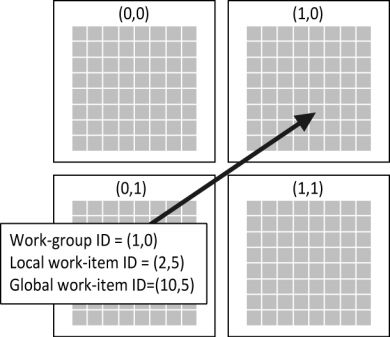
\includegraphics[width=0.50\textwidth]
	{pics/opencl-work.jpg}
	\caption{Contoh \textit{work-space} dua dimensi. \textit{Work-space} terbagi menjadi empat \textit{work-group} dua dimensi. Semua \textit{work-group} selalu memiliki ukuran yang sama.}
	\label{fig:work}
\end{figure}

Pada OpenCL terdapat batasan terhadap ukuran \textit{work-group} yang dapat digunakan untuk menjalankan suatu OpenCL \textit{kernel}. Terdapat dua jenis batasan, yaitu batasan dari \textit{device} dan batasan dari OpenCL \textit{kernel}. Setiap \textit{mobile} GPU memiliki batasan banyak maksimal \textit{work-item} yang dapat berada dalam satu \textit{work-group}. Misalnya pada beberapa Adreno GPU, banyak maksimal \textit{work-item} dalam satu \textit{work-group} adalah 1024. Setiap OpenCL \textit{kernel} juga memiliki batasan tersendiri yang ditentukan oleh kompleksitas OpenCL \textit{kernel} tersebut. Jika \textit{kernel} semakin kompleks maka banyak maksimal \textit{work-item} dalam satu \textit{work-group} akan semakin kecil. Batasan yang berasal dari OpenCL \textit{kernel} ini selalu lebih kecil atau sama dengan batasan dari \textit{device}.

\section{Jenis Memori pada OpenCL}
%-----------------------------------------------------------------------------%
Setiap \textit{work-item} yang menjalankan OpenCL \textit{kernel} dapat mengakses beberapa jenis memori \cite{opencl}. Setiap jenis memori memiliki kelebihan dan kekurangan masing-masing dalam hal latensi dan kapasitas. Berikut adalah empat jenis memori yang secara konsep terdapat pada OpenCL.

\begin{enumerate}

\item \textbf{\textit{Global Memory}}. \textit{Global memory} merupakan memori yang dapat diakses oleh seluruh \textit{work-item} pada suatu \textit{work-space}. Memori ini digunakan untuk menyimpan \textit{buffer object}. Memori ini memiliki latensi paling besar di antara empat jenis memori. Meskipun lambat, memori ini memiliki kapasitas yang paling besar dibandingkan jenis memori lain.

\item \textbf{\textit{Constant Memory}}. \textit{Constant memory} merupakan memori dengan latensi kecil. \textit{Constant memory} digunakan untuk menyimpan data-data yang bersifat konstan. Argumen-argumen OpenCL \textit{kernel} yang berupa skalar atau vektor disimpan di \textit{constant memory}. Jika suatu data konstan tidak dapat lagi disimpan di \textit{constant memory} karena sudah penuh, maka data akan disimpan di lokasi lain dan dapat menyebabkan latensinya lebih tinggi.

\item \textbf{\textit{Local Memory}}. \textit{Local memory} merupakan memori yang dapat diakses oleh semua \textit{work-item} yang berada dalam satu \textit{work-group}. Latensi dari memori ini relatif kecil. \textit{Local memory} sering digunakan untuk melakukan \textit{caching} dalam kasus ketika \textit{work-items} dalam suatu \textit{work-group} perlu mengakses data yang sama berkali-kali.

\item \textbf{\textit{Private Memory}}. Memori ini bersifat \textit{private} untuk suatu \textit{work-item} dan tidak dapat diakses oleh \textit{work-item} lain. Memori ini digunakan untuk menyimpan \textit{private variable}. Jika \textit{private memory} yang berada di \textit{regsiter} sudah penuh, maka \textit{private variable} akan disimpan di lokasi lain sehingga menyebabkan latensinya lebih tinggi.  

\end{enumerate}

Pada OpenCL \textit{kernel}, akses memori sering menjadi \textit{bottleneck}. Meminimalkan \textit{read}/\textit{write} terhadap jenis memori yang lambat dan maksimal \textit{read}/\textit{write} terhadap jenis memori yang cepat dapat membantu meningkatkan performa OpenCL \textit{kernel} secara signifikan. Secara umum \textit{local memory} dan \textit{constant memory} sangat disarankan penggunaannya \cite{opencl}.

\section{Tipe Data Vektor pada OpenCL}
%-----------------------------------------------------------------------------%
Tipe data vektor merupakan sebuah tipe data berupa vektor sepanjang $N$ yang mengandung $N$ skalar di dalamnya. Pada OpenCL, contoh tipe data vektor adalah $floatN$ yang merupakan vektor berisi $N$ buah \textit{floating point} \cite{opencl}. Nilai $N$ yang mungkin pada OpenCL adalah 2, 4, 8, dan 16. Penggunaan tipe data vektor dapat membantu mengurangi biaya operasi \textit{read}/\textit{write} terhadap memori sehingga meningkatkan performa OpenCL \textit{kernel}. Dengan menggunakan tipe data $float4$ misalnya, suatu vektor yang berisi empat buah \textit{floating point} dibaca hanya melalui satu kali instruksi. Nilai $N$ yang disarankan untuk digunakan pada tipe data vektor adalah 4. Pada beberapa jenis GPU, contohnya Adreno, untuk mengakses vektor yang panjangnya lebih dari 4 diperlukan lebih dari satu instruksi \textit{read}/\textit{write}.